\section{Experiments}

\subsection{Setup}

The experiments use SIFT1M \citep{jegou2011pq,texmexsift} and four public
ANN10M xbin subsets: BIGANN, DEEP, Microsoft Turing-ANNS, and Microsoft
SPACEV.\@ Unless stated otherwise, the task is flat squared-L2 search followed
by top-$K$ selection. The GPU baseline uses FAISS v1.14.3
\citep{faiss2026software}: cuBLAS computes squared-L2 scores, and
\texttt{runBlockSelect} performs exact top-$K$ selection. The CPU comparison
uses FAISS \texttt{IndexFlatL2::search} and \texttt{knn\_L2sqr}.

The main timing metric is end-to-end speedup: exact flat-search time divided by
Monte-Carlo TopK time, including sample scoring, filtering, candidate top-$K$,
and fallback. Selector speedup compares only exact top-$K$ selection with
Monte-Carlo TopK selection. Correctness is reported in three ways. ID overlap is
the overlap with the exact top-$K$ identifiers. Returned-score agreement checks
whether the returned $K$-th score matches exact selection. Tie-aware overlap
also accepts identifiers tied with the exact $K$-th score. Tables abbreviate
returned-score agreement and tie-aware overlap minima as ``score/tie min.''

These metrics separate correctness from tie-breaking and parameter safety. A
low ID overlap indicates an error only if the returned score boundary changes
or if tie-aware overlap also falls. If returned-score agreement and tie-aware
overlap are both 1.0, the row has an exact score boundary and the ID difference
comes from arbitrary ordering among equal-score boundary items. We therefore
also report boundary-tie counts. Separately, underflow, overflow, and fallback
counts show whether a parameter setting is safe, while candidate p99/max and
selector p99 show whether the cap and tail latency are well controlled.

The benchmark flags map to the notation in Section~\ref{sec:method} as
\texttt{sample\_n}=$m$, \texttt{sample\_k}=$r$, and
\texttt{candidate\_cap}=$C_{\max}$.

\subsection{FAISS GPU on ANN10M}

\begin{table}[!htbp]
\centering
\caption{FAISS GPU ANN10M flat-search benchmark on RTX 4090 over five sample
seeds. All rows use 1024 queries, $K=64$, \texttt{sample\_n=32768},
\texttt{sample\_k=4}, and \texttt{candidate\_cap=8192}. Speedups and candidate
means are mean/std across seeds; the p99 column gives the range across seeds.}%
\label{tab:faiss_ann10m_xbin}
\resizebox{\linewidth}{!}{%
\begin{tabular}{llrrrrrrrrrr}
\toprule
Dataset & dtype & Exact & MC & Speedup & Select speedup &
Cand.\ mean & Cand.\ p99 & ID min & Score/tie min & Tie rows/max & Fallbacks \\
\midrule
BigANN & uint8 & 1.0544 & 0.4024 & $2.620{\pm}0.002$x & $15.077{\pm}0.013$x & $1223{\pm}11$ & 2862--3052 & 0.9844 & 1.0/1.0 & 14/3 & 0 \\
Deep & float32 & 1.0081 & 0.3561 & $2.831{\pm}0.001$x & $15.073{\pm}0.009$x & $1225{\pm}7$ & 2784--3116 & 0.3438 & 1.0/1.0 & 38/191 & 0 \\
MSSPACEV & int8 & 1.0191 & 0.3672 & $2.775{\pm}0.001$x & $15.071{\pm}0.006$x & $1227{\pm}15$ & 2930--3223 & 0.1250 & 1.0/1.0 & 68/1240 & 0 \\
MSTuring & float32 & 1.0193 & 0.3676 & $2.773{\pm}0.001$x & $15.068{\pm}0.010$x & $1218{\pm}28$ & 2844--3142 & 1.0000 & 1.0/1.0 & 31/3 & 0 \\
\bottomrule
\end{tabular}%
}
\end{table}

\begin{figure}[!htbp]
\centering
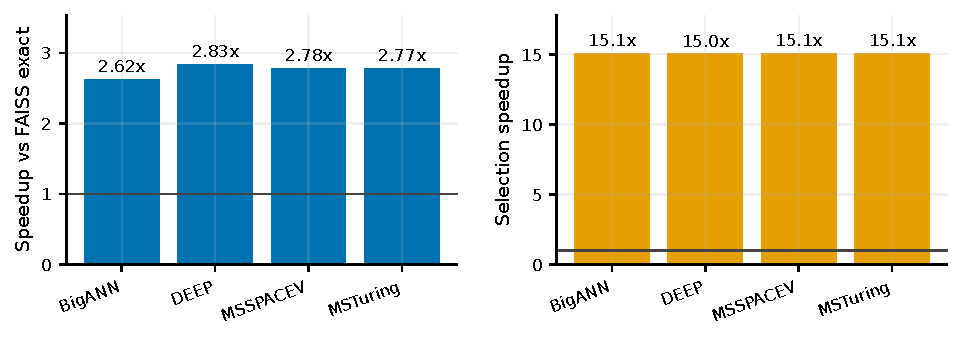
\includegraphics[width=0.90\linewidth]{figures/ann10m_gpu_speedups.pdf}
\caption{FAISS GPU ANN10M speedups. All four datasets have zero underflows,
overflows, and fallbacks across five sample seeds.}
\label{fig:ann10m_gpu_speedups}
\end{figure}

Table~\ref{tab:faiss_ann10m_xbin} and
Figure~\ref{fig:ann10m_gpu_speedups} show the main GPU result. Monte-Carlo TopK
reduces FAISS top-$K$ selection from about 0.700 s to 0.046 s, a 15.0x selector
speedup. End-to-end flat-search speedup is 2.62x--2.83x. All rows have zero
underflows, zero overflows, and zero fallbacks across five sample seeds.

The low worst-row ID overlap on Deep and MSSPACEV is caused by equal-score
boundary ties. In every row, the returned $K$-th score matches exact selection,
and the tie-aware overlap minimum is 1.0. The largest boundary tie has 191
identifiers on Deep and 1240 on MSSPACEV.\@ The observed candidate means
($1218$--$1227$) match the order-statistic estimate
$10^7\cdot4/32768=1220.7$, while the p99 range is wider than an iid model would
predict.

\begin{table}[!htbp]
\centering
\caption{GPU cap and parameter sweep on the tie-heavy ANN10M datasets
(one seed). Strict mode falls back on overflow; capped mode is approximate and
keeps at most $C_{\max}$ candidates. Capped rows use small caps to expose the quality/latency
trade-off. The $m/r/C_{\max}$ column gives sample size, sample rank, and
candidate cap. All rows use 1024 queries, $K=64$, and batch size 32.}%
\label{tab:ann10m_gpu_param_sweep}
\resizebox{\linewidth}{!}{%
\begin{tabular}{llrrrrrrrr}
\toprule
Dataset & Mode & $m/r/C_{\max}$ & Speedup & Select speedup &
Cand.\ p99/max & ID min & Score/tie min & Overflow/fallback & Select p99 \\
\midrule
Deep & strict & 32768/4/4096 & 2.834x & 15.14x & 2949/4009 & 0.4219 & 1.0/1.0 & 0/0 & 1.45 ms \\
Deep & strict & 32768/4/8192 & 2.832x & 15.08x & 2949/4009 & 0.4219 & 1.0/1.0 & 0/0 & 1.45 ms \\
Deep & strict & 65536/8/8192 & 2.809x & 14.36x & 2506/3346 & 0.4219 & 1.0/1.0 & 0/0 & 1.53 ms \\
Deep & capped & 32768/4/2048 & 2.835x & 15.18x & 2949/4009 & 0.4375 & 0.0/0.5 & 101/0 & 1.45 ms \\
Deep & capped & 32768/4/4096 & 2.835x & 15.14x & 2949/4009 & 0.4375 & 1.0/1.0 & 0/0 & 1.45 ms \\
MSSPACEV & strict & 32768/4/4096 & 0.289x & 0.22x & 3223/4354 & 0.2188 & 1.0/1.0 & 1/1 & 2182.13 ms \\
MSSPACEV & strict & 32768/4/8192 & 2.772x & 15.06x & 3223/4354 & 0.0625 & 1.0/1.0 & 0/0 & 1.45 ms \\
MSSPACEV & strict & 65536/8/8192 & 2.750x & 14.34x & 2467/3121 & 0.0625 & 1.0/1.0 & 0/0 & 1.53 ms \\
MSSPACEV & capped & 32768/4/2048 & 2.779x & 15.19x & 3223/4354 & 0.1719 & 0.0/0.5 & 115/0 & 1.44 ms \\
MSSPACEV & capped & 32768/4/4096 & 2.777x & 15.13x & 3223/4354 & 0.1094 & 0.0/0.9844 & 1/0 & 1.45 ms \\
\bottomrule
\end{tabular}%
}
\end{table}

Table~\ref{tab:ann10m_gpu_param_sweep} separates parameter tuning from tie
handling. Larger samples reduce the candidate tail: Deep p99/max drops from
2949/4009 to 2506/3346, and MSSPACEV drops from 3223/4354 to 2467/3121. The
raw ID minimum does not become 1.0 because FAISS exact selection and the
candidate selector may choose different valid identifiers from the same
boundary-score tie set. Achieving raw ID overlap 1.0 on these rows would require
a stable score--ID tie-breaker in both selectors, not a larger cap. The sweep
also explains the GPU cap choice. MSSPACEV with cap 4096 has one overflow
fallback and the selector p99 rises to 2.18 s; cap 8192 removes the fallback.
The capped rows use cap 2048 and 4096 as stress points below or near the
observed candidate maximum. Deep at cap 4096 has no overflow, so capped and
strict mode agree. MSSPACEV at cap 4096 still truncates one overflow row and
has returned-score agreement minimum 0.0. A cap of 8192 has no overflow in this
sweep, so capped mode is equivalent to the strict row and is not listed
separately.

\subsection{SIFT1M Parameter Behavior}

\begin{table}[!htbp]
\centering
\caption{FAISS SIFT1M flat-search rows on RTX 4090 using exact fallback.
Candidate statistics are p50/p95/p99/max. All rows have returned-score
agreement and tie-aware overlap 1.0.}%
\label{tab:faiss_sift1m}
\resizebox{\linewidth}{!}{%
\begin{tabular}{rrrrrrrrrr}
\toprule
Q & $K$ & \texttt{sample\_k} & Speedup & Select speedup &
ID min & Candidates & Under/over/fallback & Select p99 & Tie rows/max \\
\midrule
1024 & 64 & 4 & 2.73x & 10.25x & 0.9844 & 446/954/1166/1579 & 0/0/0 & 0.22 ms & 41/2 \\
9984 & 64 & 4 & 0.165x & 0.122x & 0.9844 & 444/956/1216/2064 & 18/0/18 & 316 ms & 455/3 \\
9984 & 64 & 8 & 2.72x & 10.02x & 0.9844 & 934/1595/1927/3203 & 0/0/0 & 0.23 ms & 455/3 \\
1024 & 1024 & 32 & 3.19x & 22.69x & 0.9990 & 3813/5066/5573/6423 & 0/0/0 & 0.32 ms & 148/3 \\
\bottomrule
\end{tabular}%
}
\end{table}

\begin{figure}[!htbp]
\centering
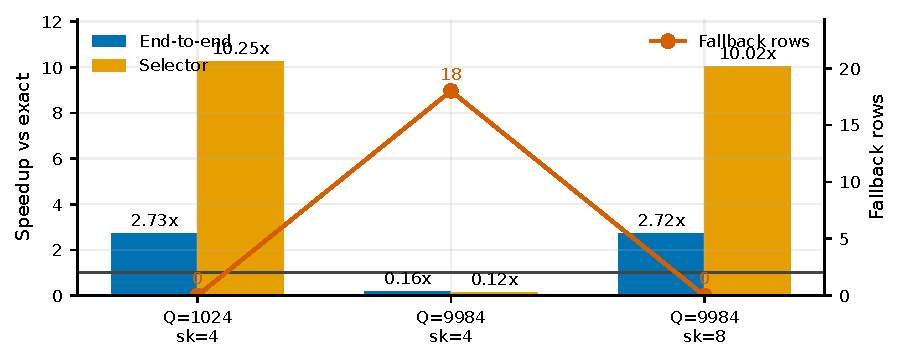
\includegraphics[width=0.84\linewidth]{figures/sift1m_fallback_region.pdf}
\caption{SIFT1M parameter behavior. The full-query \texttt{sample\_k=4} row
triggers 18 underflow fallbacks and becomes slower than exact selection, while
\texttt{sample\_k=8} avoids fallback and recovers the expected selector gain.}
\label{fig:sift1m_fallback_region}
\end{figure}

Table~\ref{tab:faiss_sift1m} and
Figure~\ref{fig:sift1m_fallback_region} show that the threshold rank must be
chosen for the tail, not only for the mean. With \texttt{sample\_k=8}, the
full-query run has zero fallbacks, a 10.02x selector speedup, and a 2.72x
end-to-end speedup. With \texttt{sample\_k=4}, 18 underflow rows fall back to
full-row exact selection, and the run becomes slower than exact top-$K$. The
practical tuning rule is therefore to avoid fallback first, then reduce the
candidate count.

\begin{figure}[!htbp]
\centering
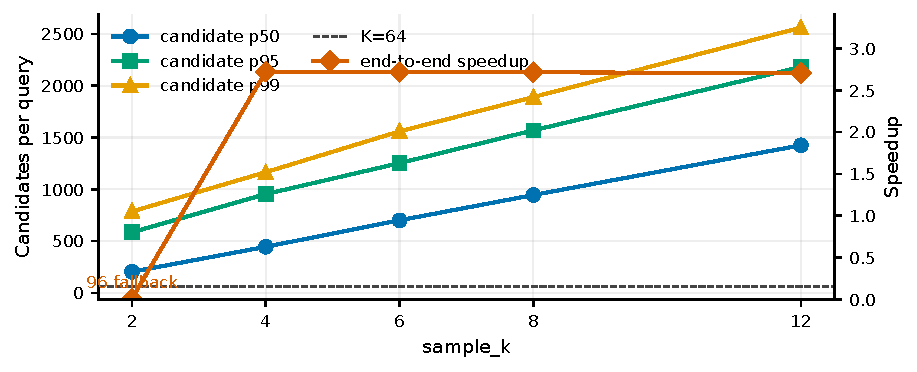
\includegraphics[width=0.84\linewidth]{figures/sift1m_samplek_candidates.pdf}
\caption{SIFT1M \texttt{sample\_k} sensitivity for 1024 queries and $K=64$.
\texttt{sample\_k=2} keeps too few candidates and triggers 96 fallbacks. Larger
values increase candidate quantiles but keep returned-score agreement and
tie-aware overlap 1.0.}
\label{fig:sift1m_samplek_candidates}
\end{figure}

\begin{figure}[!htbp]
\centering
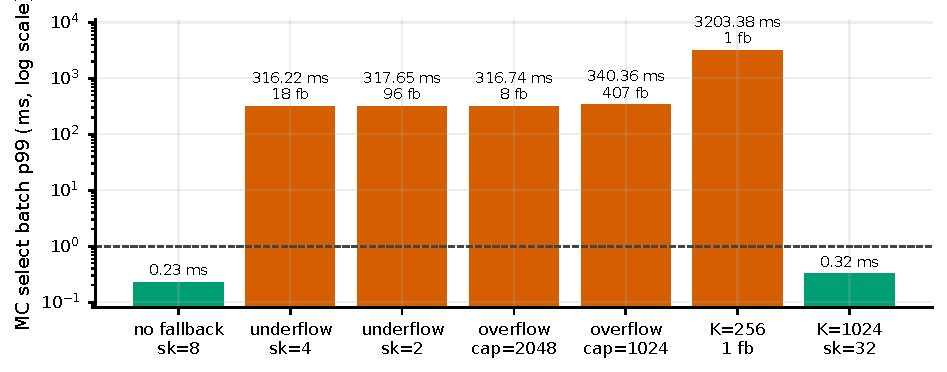
\includegraphics[width=0.84\linewidth]{figures/sift1m_tail_latency.pdf}
\caption{Tail latency is set by fallback rows. Rows without fallback have
sub-millisecond MC select p99, while underflow or overflow fallback pushes p99
to hundreds of milliseconds; one $K=256$ underflow row raises p99 above 3 s.}
\label{fig:sift1m_tail_latency}
\end{figure}

\begin{figure}[!htbp]
\centering
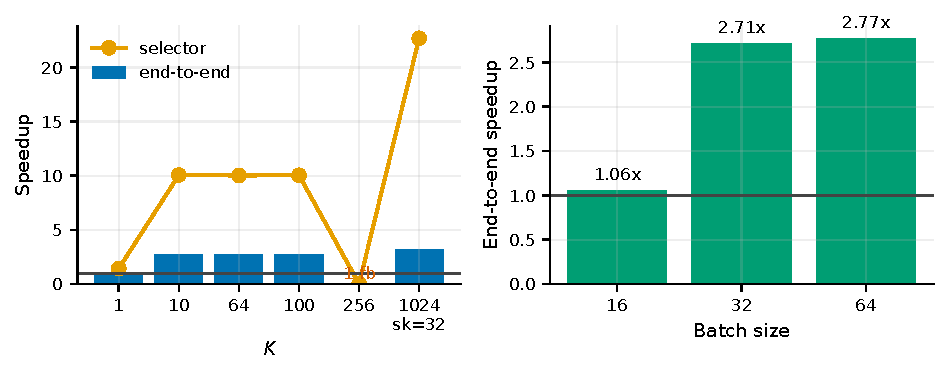
\includegraphics[width=0.84\linewidth]{figures/sift1m_k_batch_sensitivity.pdf}
\caption{Extra SIFT1M sensitivity. $K=1$ leaves little selection time to save;
$K=1024$ requires a larger threshold rank (\texttt{sample\_k=32}) to avoid
underflow and then recovers 3.19x end-to-end speedup. Batch-size results show
that throughput and sample scoring can shift the end-to-end gain.}
\label{fig:sift1m_k_batch_sensitivity}
\end{figure}

Figures~\ref{fig:sift1m_samplek_candidates},
\ref{fig:sift1m_tail_latency}, and
\ref{fig:sift1m_k_batch_sensitivity} show the same pattern in sweeps over
\texttt{sample\_k}, $K$, and batch size. Fallback rows dominate tail latency.
In no-fallback rows, the selector p99 is below 0.4 ms in these SIFT1M runs.

\subsection{CPU and Capped Mode}

Table~\ref{tab:faiss_cpu_ann10m} shows the CPU result. Monte-Carlo TopK is
1.85--3.12x faster than FAISS \texttt{IndexFlatL2::search} and 2.00--3.29x
faster than \texttt{knn\_L2sqr}, with exact top-$K$ agreement and zero
fallbacks.

\begin{table}[!htbp]
\centering
\caption{FAISS CPU ANN10M comparison on an Intel Core i9-13900KF.\@ All rows use
1024 queries, $K=64$, \texttt{sample\_n=32768}, \texttt{sample\_k=4}, and
\texttt{candidate\_cap=8192}. Times are seconds.}%
\label{tab:faiss_cpu_ann10m}
\resizebox{\linewidth}{!}{%
\begin{tabular}{llrrrrrr}
\toprule
Dataset & dtype & IndexFlatL2 & \texttt{knn\_L2sqr} & MC total &
IndexFlat/MC & \texttt{knn}/MC & ID overlap \\
\midrule
BigANN & uint8 & 21.773 & 22.992 & 6.985 & 3.12x & 3.29x & 1.000 \\
Deep & float32 & 16.022 & 17.032 & 5.772 & 2.78x & 2.95x & 1.000 \\
MSSPACEV & int8 & 11.692 & 12.269 & 5.985 & 1.95x & 2.05x & 1.000 \\
MSTuring & float32 & 11.099 & 12.016 & 6.008 & 1.85x & 2.00x & 1.000 \\
\bottomrule
\end{tabular}%
}
\end{table}

\begin{table}[!htbp]
\centering
\caption{FAISS overflow-capping stress test based on SIFT1M. Effective 10M rows
repeat the SIFT1M score matrix; they are not physical 10M dataset runs.
Candidates are mean/min/max.}%
\label{tab:faiss_overflow_capping}
\resizebox{\linewidth}{!}{%
\begin{tabular}{rrrrrrrrr}
\toprule
Effective $N$ & Cap & MC total & Phys.\ speedup & Select speedup &
ID overlap mean/min & Candidates & Overflows & Fallbacks \\
\midrule
1M & 256 & 0.0348 & 2.92x & 14.88x & 0.6112/0.0625 & 490/66/1579 & 863 & 0 \\
10M & 2048 & 0.1222 & 2.92x & 15.74x & 0.5542/0.0938 & 4902/660/15790 & 935 & 0 \\
10M & 4096 & 0.1226 & 2.92x & 15.63x & 0.8540/0.2031 & 4902/660/15790 & 589 & 0 \\
10M & 8192 & 0.1231 & 2.91x & 15.46x & 0.9901/0.5313 & 4902/660/15790 & 106 & 0 \\
10M & 16384 & 0.1232 & 2.91x & 15.33x & 1.0000/0.9844 & 4902/660/15790 & 0 & 0 \\
\bottomrule
\end{tabular}%
}
\end{table}

\begin{figure}[!htbp]
\centering
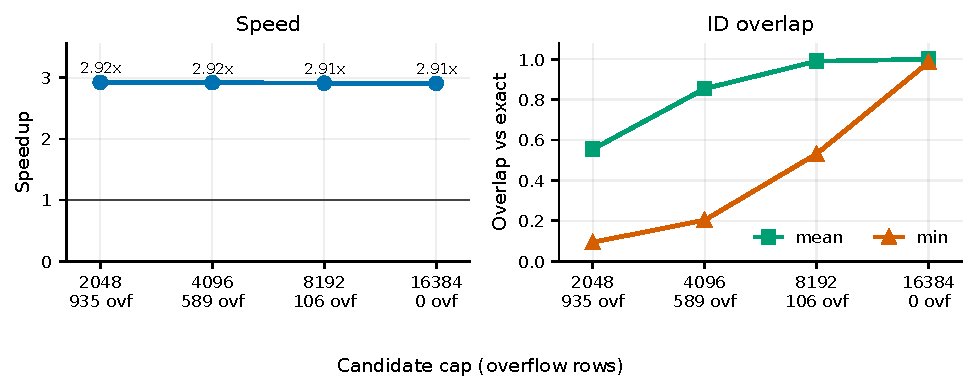
\includegraphics[width=0.90\linewidth]{figures/overflow_capping_tradeoff.pdf}
\caption{Overflow capping bounds selector work but loses overlap. The plotted
rows use the effective 10M repeated-score stress case.}
\label{fig:overflow_capping_tradeoff}
\end{figure}

\FloatBarrier

Table~\ref{tab:faiss_overflow_capping} and
Figure~\ref{fig:overflow_capping_tradeoff} isolate the approximate capped mode.
At effective $N=10$M, cap 8192 keeps selector speedup near 15.5x and mean ID
overlap at 0.9901, but worst-row overlap is only 0.5313. Cap 16384 removes
overflows and raises worst-row overlap to 0.9844. These rows are stress tests
for the selector, not physical 10M end-to-end retrieval results.
